\documentclass[12pt,a4paper]{article}
\usepackage[utf8]{inputenc}
\usepackage[german]{babel}
\usepackage[T1]{fontenc}
\usepackage{amsmath}
\usepackage{amsfonts}
\usepackage{amssymb}
\usepackage{graphicx}
\usepackage{float}
\usepackage[left=2cm,right=2cm,top=2cm,bottom=2cm]{geometry}
\usepackage{siunitx}
\author{Moritz}

\begin{document}
\setlength{\parindent}{0pt} 
\begin{center}
{\LARGE Versuchsprotokoll}\\
\begin{large}
zum Grundpraktikum Physik Teil I\\[0.4cm]
an der RWTH Aachen\\
I. Physikalisches Institut B\\[4.5cm]
\Large\textbf{\textsl{Mechanik}}\\[4cm]
\normalsize\textit{vorgelegt\\von}\\[0.4cm]
\large{Moritz Berger\\Tim Herbermann\\Gerald Kolter\\Sebastian Siebert}\\[1cm]
\large \textit{Gruppe B07} \\ [3cm]
\large \textbf{Wintersemester 2016/2017}
\end{large}
\end{center}
\newpage

\tableofcontents
\newpage

\part{Trägheitsmomente}

\section{Grundlagen}
In diesem Versuch soll das Trägheitsmoment verschiedener Körper analysiert werden.\\
Dieses ist allgemein definiert über
\begin{equation}
J = \int r^2\cdot dm
\end{equation}.
Wir werden das Trägheitsmoment aus der Schwingungsdauer einer Drillachse, die durch eine Spiralfeder zum schwingen gebracht wird, bestimmen. Dabei wird ein Zusammenhang zwischen Schwingungsperiode T und dem Trägheitsmoment J  aus der Definition des Drehmomentes M hergeleitet:
\begin{equation}
M = J\cdot \dot{\omega}\Rightarrow -D\cdot \phi = J\cdot \ddot{\phi}\Rightarrow \ddot{\phi} + \dfrac{D}{J}\cdot \phi = 0
\end{equation}
Die Lösung dieser Differentialgleichung ist eine harmonische Schwingung mit der Kreisfrequenz $\omega = \sqrt{\dfrac{D}{J}}$. Daraus folgt:
\begin{equation}
 T = 2\cdot \pi \sqrt{\dfrac{J}{D}}
\end{equation}
oder, falls man das Trägheitsmoment angeben möchte:
\begin{equation}
J = \dfrac{D}{4\cdot \pi^2}\cdot T^2
\end{equation}\\
\\
Der Versuch wird in drei Teile aufgeteilt.\\
Im ersten Teil soll das Trägheitsmoment von Massenpunkten in Abhängigkeit von dem Abstand zur Drehachse untersucht werden. Dabei wird als erstes das von der Feder bestimmte Direktionsmoment D bestimmt.\\
Im zweiten Teil wird das Trägheitsmoment eines Hohlzylinders, eines Vollzylinders, einer Kugel und einer Kreisscheibe miteinander verglichen.\\
Im dritten Teil soll der Steinersche Satz
\begin{equation}
J = J_0+m*R^2
\end{equation}
bestätigt werden.

\section{Aufbau und Durchführung}
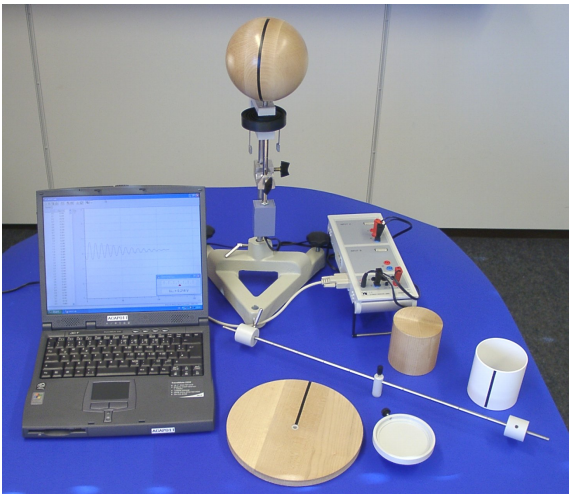
\includegraphics[width=\linewidth]{Bilder/Aufbau.PNG}
Der grundsätzliche Aufbau der drei Teilversuche ist gleich. Es wird ein kugelgelagterter Stab mit einem Stativ und mit einer Spiralfeder, die eine Schwingung erzeugen soll, befestigt. Am unteren Stabende werden an der Innenseite einer U-förmigen Gabel zwei Magnete so befestigt, dass sich Nord- und Südpol gegenüber liegen. Zwischen die Magnete wird eine Hallsonde geführt, die durch eine Magnetfeldänderung die Schwingung registrieren soll. Sie wird mit der Spannungsquelle des CASSYs verbunden. Die entstehende Hall-Spannung wird ebenfalls mit dem CASSY gemessen. Auf den Stab können je nach Teilversuch verschiedene Aufsätze aufgesetzt werden.\\
\\
Vor dem experimentieren wird die Hallsonde durch horizontales Drehen so justiert, dass die gemessene Spannung möglichst bei \SI{0}{V} liegt.
\section{Bestimmung des Direktionsmomentes}

\section{Vergleich von Trägheitsmomenten}

\section{Bestätigung des Steinerschen Satzes}

\end{document}